\documentclass[border=6pt]{standalone}
\usepackage[T1]{fontenc}
\usepackage{mathptmx}
\usepackage{tikz}
\usetikzlibrary{positioning,arrows.meta}
\definecolor{navy}{HTML}{1F3A5F}\definecolor{acc}{HTML}{D9622B}\definecolor{band}{HTML}{DCE3EC}\definecolor{grn}{HTML}{1B8A5A}
\begin{document}
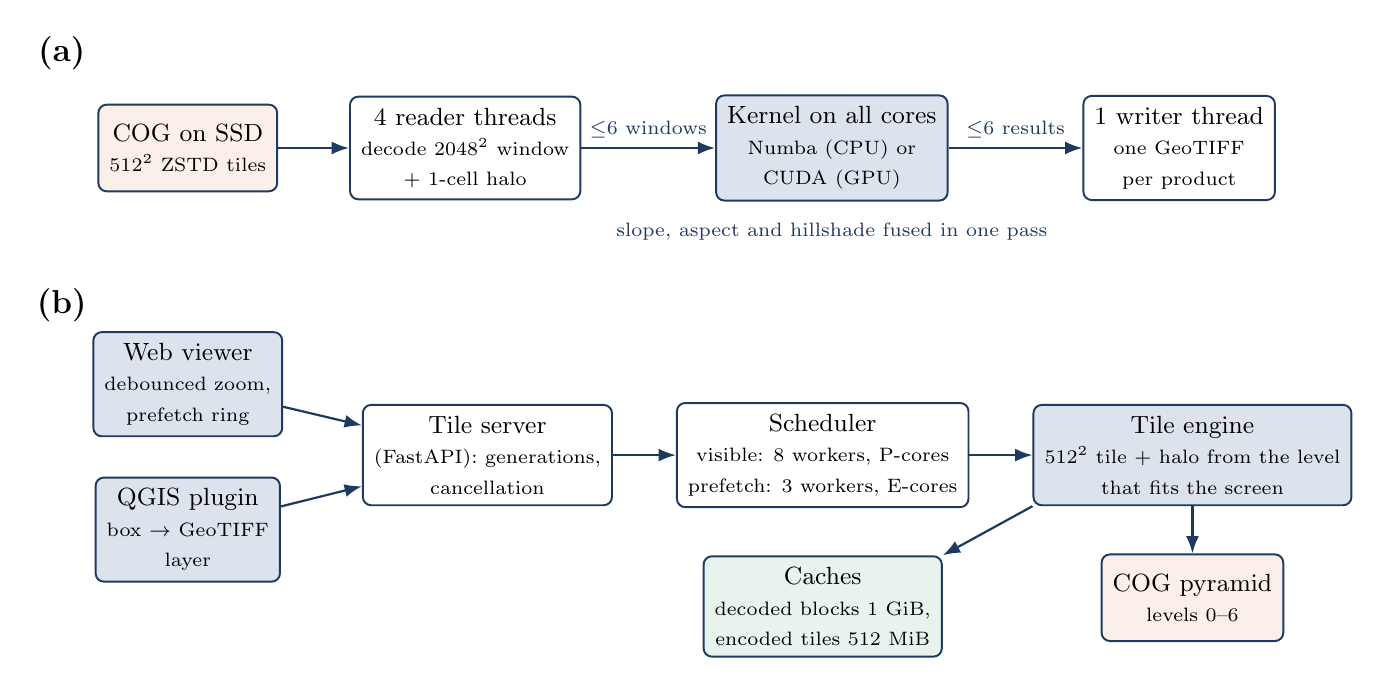
\begin{tikzpicture}[font=\small, box/.style={draw=navy, rounded corners=3pt, align=center, minimum height=11mm,
  inner sep=4pt, fill=white, line width=0.7pt},
  arr/.style={-{Latex[length=2.2mm]}, navy, line width=0.8pt}, lab/.style={font=\bfseries\large}]
% (a) whole-grid engine
\node[lab] at (-0.7,1.2) {(a)};
\node[box, fill=acc!10] (cog) at (0.9,0) {COG on SSD\\{\scriptsize 512$^2$ ZSTD tiles}};
\node[box, right=9mm of cog] (rd) {4 reader threads\\{\scriptsize decode 2048$^2$ window}\\{\scriptsize + 1-cell halo}};
\node[box, right=17mm of rd, fill=band] (k) {Kernel on all cores\\{\scriptsize Numba (CPU) or}\\{\scriptsize CUDA (GPU)}};
\node[box, right=17mm of k] (wr) {1 writer thread\\{\scriptsize one GeoTIFF}\\{\scriptsize per product}};
\draw[arr] (cog)--(rd);
\draw[arr] (rd)--node[above,font=\scriptsize]{$\le$6 windows}(k);
\draw[arr] (k)--node[above,font=\scriptsize]{$\le$6 results}(wr);
\node[font=\scriptsize, text=navy, below=1.5mm of k] {slope, aspect and hillshade fused in one pass};
% (b) viewer system
\node[lab] at (-0.7,-2.0) {(b)};
\node[box, fill=band] (web) at (0.9,-3.0) {Web viewer\\{\scriptsize debounced zoom,}\\{\scriptsize prefetch ring}};
\node[box, fill=band, below=5mm of web] (qg) {QGIS plugin\\{\scriptsize box $\to$ GeoTIFF}\\{\scriptsize layer}};
\node[box, right=10mm of web, yshift=-9mm] (srv) {Tile server\\{\scriptsize (FastAPI): generations,}\\{\scriptsize cancellation}};
\node[box, right=8mm of srv] (sch) {Scheduler\\{\scriptsize visible: 8 workers, P-cores}\\{\scriptsize prefetch: 3 workers, E-cores}};
\node[box, right=8mm of sch, fill=band] (eng) {Tile engine\\{\scriptsize 512$^2$ tile + halo from the level}\\{\scriptsize that fits the screen}};
\node[box, below=6mm of sch, fill=grn!10] (cache) {Caches\\{\scriptsize decoded blocks 1 GiB,}\\{\scriptsize encoded tiles 512 MiB}};
\node[box, below=6mm of eng, fill=acc!10] (pyr) {COG pyramid\\{\scriptsize levels 0--6}};
\draw[arr] (web)--(srv); \draw[arr] (qg)--(srv); \draw[arr] (srv)--(sch); \draw[arr] (sch)--(eng);
\draw[arr] (eng)--(pyr); \draw[arr] (eng.south west)--(cache.north east);
\end{tikzpicture}
\end{document}
